\section{Matériel expérimental supplémentaire V4}
\label{sec:v4-supplement}

\subsection{Distribution des codes de décision — Campagne A}
\begin{figure}[!t]
\centering
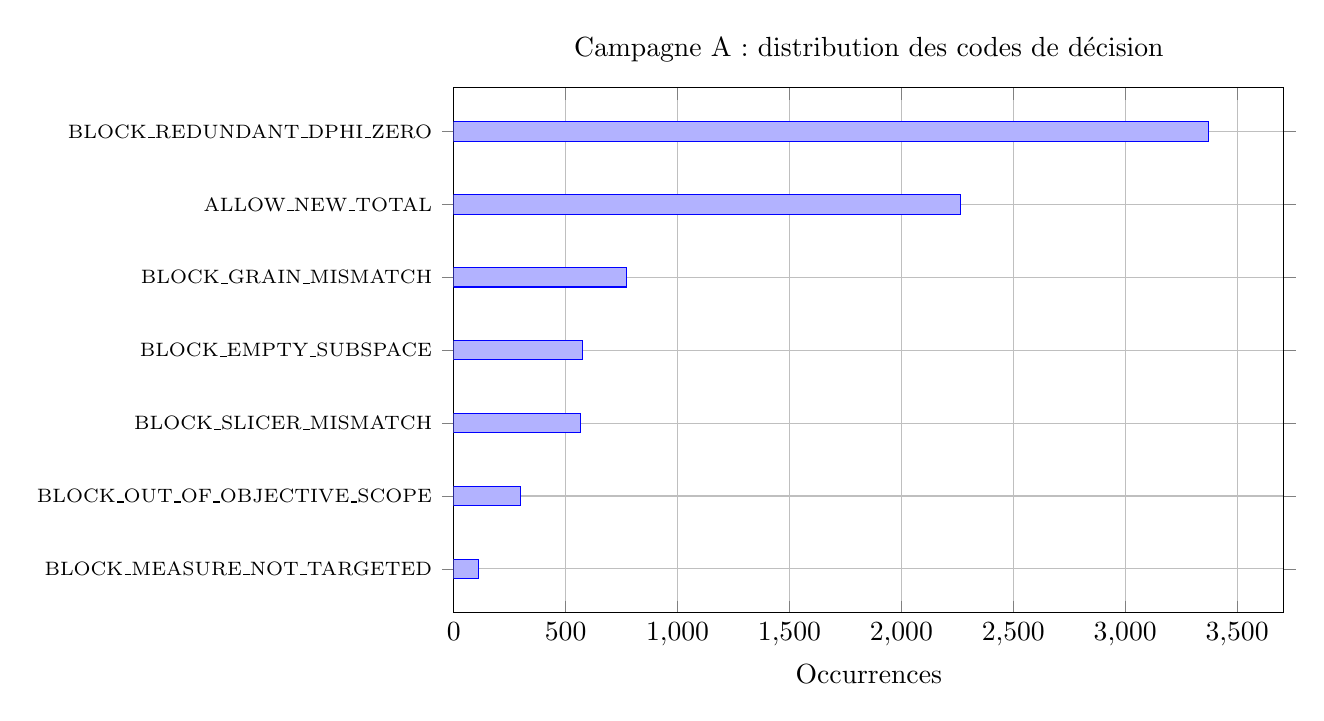
\begin{tikzpicture}
\begin{axis}[xbar,
bar width=7pt,
width=\linewidth,
height=0.68\linewidth,
title={Campagne A : distribution des codes de décision},
xlabel={Occurrences},
ytick={0,1,2,3,4,5,6},
yticklabels={{BLOCK\_MEASURE\_NOT\_TARGETED},{BLOCK\_OUT\_OF\_OBJECTIVE\_SCOPE},{BLOCK\_SLICER\_MISMATCH},{BLOCK\_EMPTY\_SUBSPACE},{BLOCK\_GRAIN\_MISMATCH},{ALLOW\_NEW\_TOTAL},{BLOCK\_REDUNDANT\_DPHI\_ZERO}},
y tick label style={font=\scriptsize},
grid=major,
xmin=0]
\addplot+ coordinates {(110,0) (300,1) (566,2) (576,3) (770,4) (2266,5) (3372,6)};
\end{axis}
\end{tikzpicture}

\caption{Répartition des codes de décision dans la Campagne A.}
\end{figure}

\subsection{Evidence usefulness — AUC}
\begin{figure}[!t]
\centering
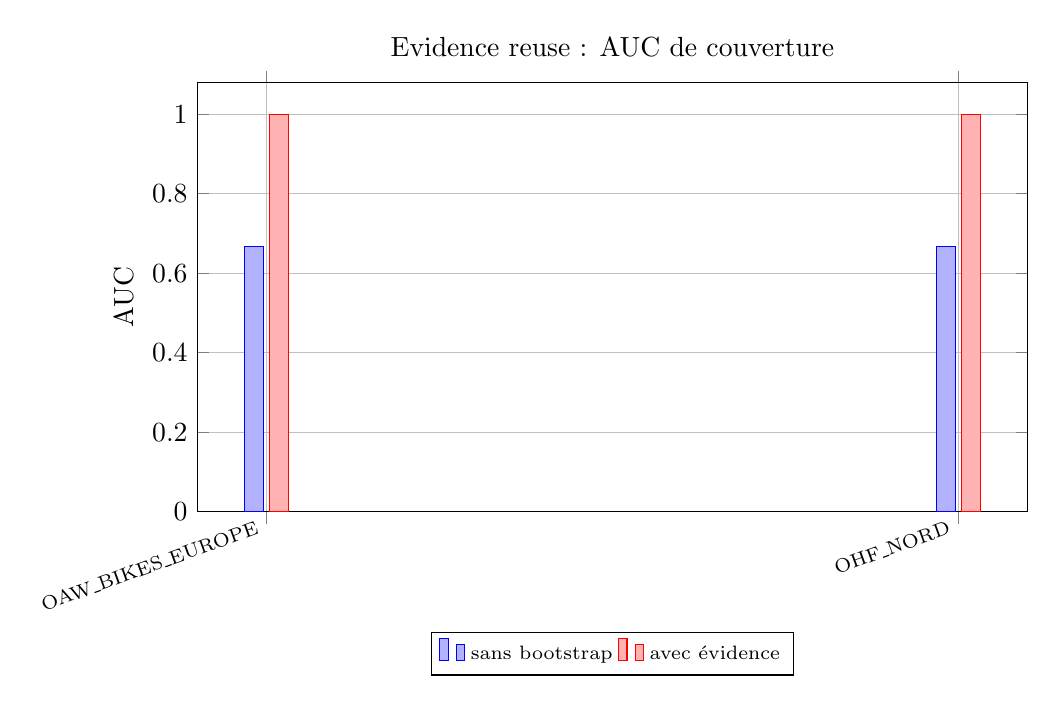
\begin{tikzpicture}
\begin{axis}[ybar,
bar width=7pt,
width=\linewidth,
height=0.58\linewidth,
title={Evidence reuse : AUC de couverture},
ylabel={AUC},
xtick={0,1},
xticklabels={{OAW\_BIKES\_EUROPE},{OHF\_NORD}},
x tick label style={rotate=20,anchor=east,font=\scriptsize},
grid=major,
legend style={font=\scriptsize,at={(0.5,-0.28)},anchor=north,legend columns=2},
ymin=0,
ymax=1.08]
\addplot+ coordinates {(0,0.666667) (1,0.666667)};
\addlegendentry{sans bootstrap}
\addplot+ coordinates {(0,1.0) (1,1.0)};
\addlegendentry{avec évidence}
\end{axis}
\end{tikzpicture}

\caption{AUC de couverture dans le petit protocole contrôlé d'utilité de l'évidence.}
\end{figure}

\subsection{Diagnostics de précision des sensibilités}
Ces figures représentent des diagnostics de précision (demi-largeurs relatives
d'intervalles de confiance) et ne sont pas utilisées comme revendications de
latence backend ou de performance industrielle.

\begin{figure}[!t]
\centering
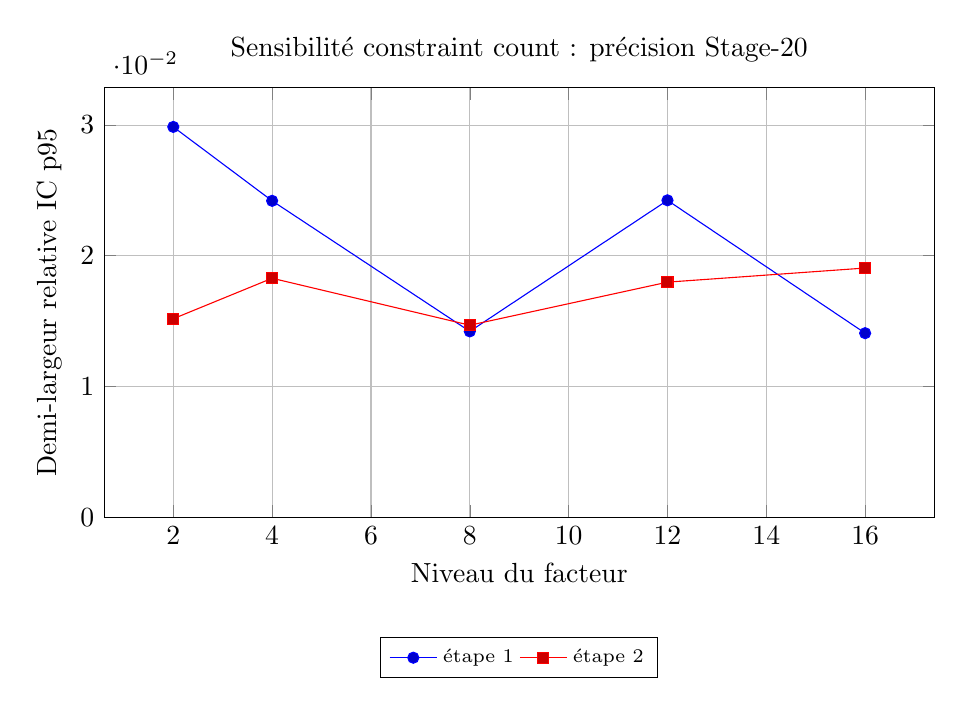
\begin{tikzpicture}
\begin{axis}[width=\linewidth,
height=0.58\linewidth,
title={Sensibilité constraint count : précision Stage-20},
xlabel={Niveau du facteur},
ylabel={Demi-largeur relative IC p95},
grid=major,
legend style={font=\scriptsize,at={(0.5,-0.28)},anchor=north,legend columns=2},
ymin=0]
\addplot+[mark=*] coordinates {(2.0,0.02986000137861953) (4.0,0.02420195483336553) (8.0,0.014211446509459035) (12.0,0.02424101696366615) (16.0,0.014073779021601897)};
\addlegendentry{étape 1}
\addplot+[mark=square*] coordinates {(2.0,0.015179910923108341) (4.0,0.018277528664099717) (8.0,0.014683287087945808) (12.0,0.017979856939250968) (16.0,0.01905925110471172)};
\addlegendentry{étape 2}
\end{axis}
\end{tikzpicture}

\caption{Diagnostic de précision de la campagne \texttt{constraint\_count}, Stage-20.}
\end{figure}

\begin{figure}[!t]
\centering
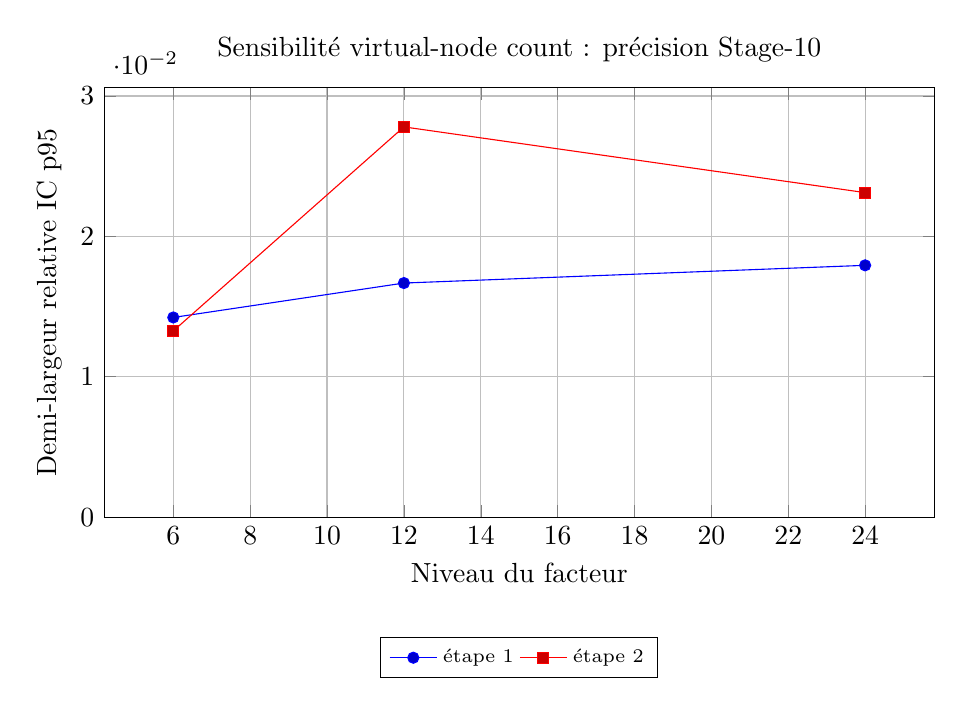
\begin{tikzpicture}
\begin{axis}[width=\linewidth,
height=0.58\linewidth,
title={Sensibilité virtual-node count : précision Stage-10},
xlabel={Niveau du facteur},
ylabel={Demi-largeur relative IC p95},
grid=major,
legend style={font=\scriptsize,at={(0.5,-0.28)},anchor=north,legend columns=2},
ymin=0]
\addplot+[mark=*] coordinates {(6.0,0.014224603883711424) (12.0,0.016675873320203795) (24.0,0.017938439828675615)};
\addlegendentry{étape 1}
\addplot+[mark=square*] coordinates {(6.0,0.013265607159975728) (12.0,0.02780124142449081) (24.0,0.023118318486393095)};
\addlegendentry{étape 2}
\end{axis}
\end{tikzpicture}

\caption{Diagnostic de précision de la campagne \texttt{virtual\_node\_count}, Stage-10.}
\end{figure}

\begin{figure}[!t]
\centering
\begin{tikzpicture}
\begin{axis}[width=\linewidth,
height=0.58\linewidth,
title={Sensibilité membership density : précision Stage-10},
xlabel={Densité (%)},
ylabel={Demi-largeur relative IC},
grid=major,
legend style={font=\scriptsize,at={(0.5,-0.28)},anchor=north,legend columns=2},
xtick={25,50,75,100},
ymin=0]
\addplot+[mark=*] coordinates {(25.0,0.006101422311198159) (50.0,0.006566516903570908) (75.0,0.006595077110573776) (100.0,0.006613480513338569)};
\addlegendentry{médiane}
\addplot+[mark=square*] coordinates {(25.0,0.023700583596975716) (50.0,0.01864639393019678) (75.0,0.015337323961677085) (100.0,0.01984926325121557)};
\addlegendentry{p95}
\end{axis}
\end{tikzpicture}

\caption{Diagnostic de précision de la campagne \texttt{membership\_density}, Stage-10.}
\end{figure}

\subsection{Traçabilité}
\begin{figure}[!t]
\centering
\resizebox{\linewidth}{!}{\begin{tikzpicture}[
node distance=4mm,
every node/.style={font=\scriptsize,align=center},
box/.style={draw,rounded corners=1mm,minimum width=18mm,minimum height=8mm,inner sep=2pt},
>=Stealth
]
\node[box] (a) {Audit};
\node[box,right=of a] (v) {Validation};
\node[box,right=of v] (f) {Freeze};
\node[box,right=of f] (ar) {Archive};
\node[box,right=of ar] (p) {Publication};
\draw[->] (a)--(v);
\draw[->] (v)--(f);
\draw[->] (f)--(ar);
\draw[->] (ar)--(p);
\node[below=5mm of f,font=\scriptsize,align=center] {manifeste + provenance + SHA-256\\source-map + claim-evidence map};
\end{tikzpicture}
}
\caption{Discipline de production des preuves : Audit $\rightarrow$ Validation $\rightarrow$ Freeze $\rightarrow$ Archive $\rightarrow$ Publication.}
\end{figure}
